\documentclass[10pt]{article}
\usepackage[utf8]{inputenc}
\usepackage{graphicx}
\usepackage{hyperref}
\usepackage{fontenc}
\usepackage{mathptmx}
\usepackage{geometry}
\usepackage{titling}
\setlength{\topskip}{0mm}
\setlength{\droptitle}{-8em} 
\title{{\large\textbf{\normalsize PROBLEM 5: CODE REVIEW : CODACY TOOL & Manual Analysis}}}
\section*{{REPOSITORY DETAILS}}
{{\normalsize https://github.com/ManushreeMallaraju/Manushree-SOEN\_6011\_Project
\\
code review comments : https://github.com/ManushreeMallaraju/Manushree-SOEN\_6011\_Project/commit/644f7c0e4252687f9eff95e4a341812460c38c84}}
 
\begin{document}
\section*{{PROBLEM 5: Code Review : CODACY Tool and Manual Analysis}}
    I did the code review of Hina's F7 source code. The review were based on the four aspects: General, Requirements Coverage, Security and Documentation with reference from Google Coding Standards. The below summary includes all my code review as a report.

\section*{\normalsize Summary of Code Review}
\\$\bullet$~ \textbf{General} : 
The source code compiles and provides an interface to give the inputs based on the users choice.  There are outputs which are printed which are not necessary. In few cases the output is not immediately displayed but it is displayed after few intermediate values are printed.
\begin{figure}[h]
\graphicspath{ {./Function6/}}
  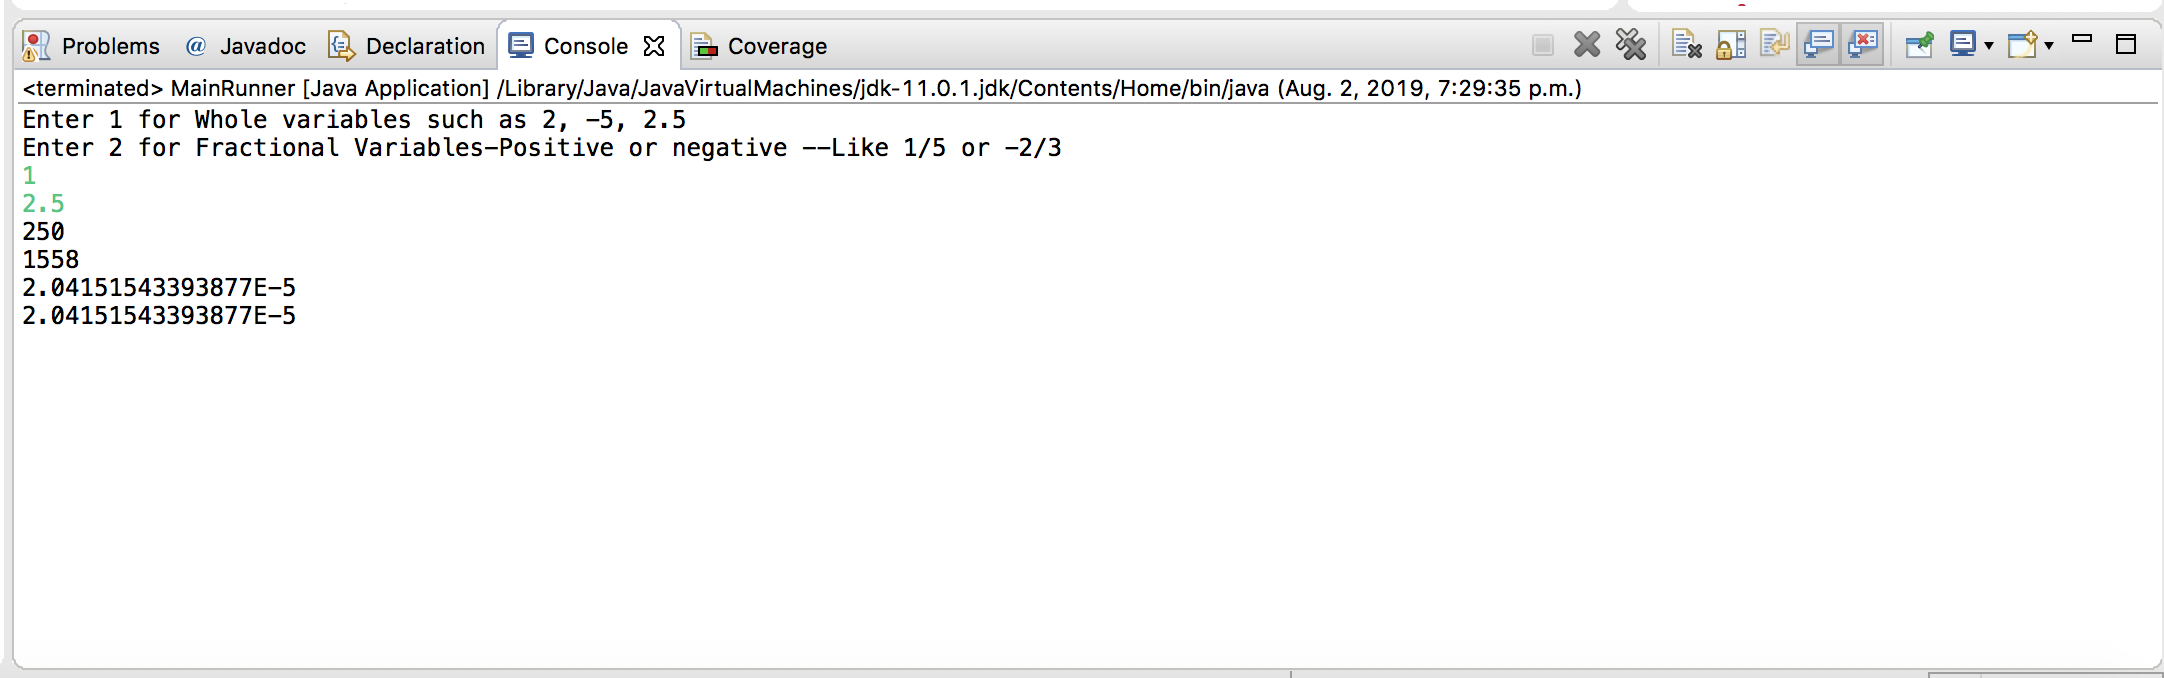
\includegraphics[width=1.0\textwidth]{SS.png}

\end{figure}
\\
\\$\bullet$~ \textbf{Requirements Coverage} : 
Code covers all the requirements and provides necessary output for the given inputs. 
\\
$\bullet$~ \textbf{Security} :
The code does not support exception handling when a user gives and improper input.
\\
$\bullet$~ \textbf{Documentation} : 
Comments are provided but needs more comments at necessary places to understand the flow of the code. Few cases where the indentation is missed as per Google Coding Standards.

\section*{\normalsize References}
https://en.wikipedia.org/wiki/Code_review
\\
https://medium.com/palantir/code-review-best-practices-19e02780015f



\end{document}